\documentclass[protokol.tex]{subfiles}
\begin{document}

\subsection*{Hodnoty}
Podmínky měření jsou uvedeny v následující tabulce.
\begin{table}[H] \label{tab:podminky}
\centering
\setlength{\tabcolsep}{10pt}
\begin{tabular}{ccc}                                                    \toprule
Teplota                 &   Tlak                    &   Vlhkost     \\
$[\si{\degreeCelsius}]$ &   $[\si{\hecto\pascal}]$  &   [\% RH]     \\  \midrule
25,3                    &   984,5                   &   29,8        \\  \bottomrule
\end{tabular}
\caption{Podmínky měření}
\end{table}

Délka provázku fyzického kyvadla byla změřena pásovým měřidlem.
\begin{table}[H] 
\centering
\setlength{\tabcolsep}{10pt}
\begin{tabular}{ccccccc}																											\toprule
							&	1		&	2		&	průměr	& 	$\sigma_{stat}$	&	$\sigma_{sys}$		&	$\sigma_{abs}$	\\	\midrule
$l \ [\si{\milli\metre}]$	&	997 	&	998		&	997,5	&	0,5  			&	0,02				&	0,5				\\ 	\bottomrule
\end{tabular}

\caption{Délka provázku pro fyzické kyvadlo}
\label{tab:delka_provazku}
\end{table}

\newpage

Průměr kuličky byl měřen posuvným měřidlem z různých stran.
\begin{table}[H] 
\centering
\setlength{\tabcolsep}{10pt}
\begin{tabular}{cccccccccc}															\toprule
							&	1	&	2	&	3	&	4	&	5	&	průměr	&	$\sigma_{stat}$		&	$\sigma_{sys}$		&	$\sigma_{abs}$	\\	\midrule
$d_k [\si{\milli\metre}]$	&	25,6&	25,2&	26,0&	25,2&	25,2&	25,4	&	0,2					&	0,02				&	0,2				\\	
$R [\si{\milli\metre}]$		&	12,8&	12,6&	13,0&	12,6&	12,6&	12,7	&	0,1					&	0,01				&	0,1				\\ \bottomrule
\end{tabular}
\caption{Rozměry kuličky}
\label{tab:rozmer_kulicky}
\end{table}

Hmotnost kuličky $m_k$ a hmotnost provázku $m_t$ byly měřeny na digitálních váhách.
$$ m_k = (62,3365 \pm 0,0001) \ \si{\gram} $$
$$ m_t = (0,5493  \pm 0,0001) \ \si{\gram} $$

Redukovaná délka reverzního kyvadla byla měřena pásovým měřidlem.
$$ l_r = (994 \pm 1) \ \si{\milli\metre} $$

Perioda fyzického kyvadla byla měřena automatickým měřičem času.
\begin{table}[H] 
\centering
\setlength{\tabcolsep}{20pt}
\begin{tabular}{ccc}												\toprule
				&	$8 T_f$				&	$T_f$				\\
				&	$[\si{\second}]$	&	$[\si{\second}]$	\\	\midrule
1				&	16,0867				&	2,0108				\\
2				&	16,0918				&	2,0115				\\
3				&	16,0924				&	2,0116				\\
4				&	16,0899				&	2,0112				\\
5				&	16,0912				&	2,0114				\\
6				&	16,0877				&	2,0110				\\
7				&	16,0904				&	2,0113				\\
8				&	16,0811				&	2,0101				\\
9				&	16,0818				&	2,0102				\\
10				&	16,0898				&	2,0112				\\	\midrule[0.5pt]
průměr			&	16,0883				&	2,0110				\\
$\sigma_{stat}$	&	0,0013				&	0,0002				\\
$\sigma_{sys}$	&	0,0001				&	0,00001				\\
$\sigma_{abs}$	&	0,0013				&	0,0002				\\	\bottomrule
\end{tabular}

\caption{Periody fyzického kyvadla}
\label{tab:periody_fyz_kyv}
\end{table}

\newpage

Následující tabulka udává periody kmitání reverzního kyvadla s čočkou dole ($T_d$) a nahoře ($T_n$) v závislosti na vzdálenosti čočky od bližšího břitu $d_z$.
\begin{table}[H] 
\centering
\setlength{\tabcolsep}{10pt}
\begin{tabular}{ccccccc}																																					\toprule
						&	\multicolumn{3}{c}{$8 T_d$}											&	\multicolumn{3}{c}{$8 T_n$}											\\
							\cmidrule(l){2-4}														\cmidrule(l){5-7}		
$d_z$					&	1					&	2					&	průměr				&	1					&	2					&	průměr				\\
$[\si{\milli\metre}]$	&	$[\si{\second}]$	&	$[\si{\second}]$	&	$[\si{\second}]$	&	$[\si{\second}]$	&	$[\si{\second}]$	&	$[\si{\second}]$	\\	\midrule
78,40					&	16,0835				&	16,0816				&	16,0826				&	16,3454				&	16,3470				&	16,3462				\\
76,32					&	16,0651				&	16,0678				&	16,0665				&	16,2764				&	16,2695				&	16,2730				\\
73,24					&	16,0472				&	16,0486				&	16,0479				&	16,1369				&	16,1384				&	16,1377				\\
71,02					&	16,0307				&	16,0325				&	16,0316				&	16,0465				&	16,0522				&	16,0494				\\
69,58					&	16,0271				&	16,0281				&	16,0276				&	15,9829				&	15,9800				&	15,9815				\\
67,40					&	16,0149				&	16,0127				&	16,0138				&	15,9135				&	15,9142				&	15,9139				\\	\bottomrule

\end{tabular}
\caption{Osminásobky period reverzního kyvadla při různých polohách čočky}
\label{tab:periody_rev_kyv}
\end{table}

Společná perioda reverzního kyvadla pro obě osy byla měřena automatickým měřičem času.
\begin{table}[H] 
\centering
\setlength{\tabcolsep}{10pt}
\begin{comment}
\begin{tabular}{ccccccccccc}										\toprule
						&	1		&	2		&	3		&	4		&	5		&	6		&	průměr	&	$\sigma_{stat}$		&	$\sigma_{sys}$	&	$\sigma_{abs}$	\\	\midrule
$8T [\si{\second}]$		&	16,0307	&	16,0308	&		&		&		&	16,0307	&	16,0308	&	0,0002				&	0,0001			&	0,0002			\\	
$T [\si{\second}]$		&	2,0038	&	2,0039	&	2,0039	&	2,0039	&	2,0038	&	2,0038	&	2,00385	&	0,00003				&	0,00001			&	0,00003			\\	\bottomrule
\end{tabular}\end{comment}

\begin{tabular}{ccc}												\toprule
				&	$8 T$				&	$T$				\\
				&	$[\si{\second}]$	&	$[\si{\second}]$	\\	\midrule
1				&	16,0307				&	2,0038				\\
2				&	16,0308				&	2,0039				\\
3				&	16,0310				&	2,0039				\\
4				&	16,0315				&	2,0039				\\
5				&	16,0300				&	2,0038				\\
6				&	16,0307				&	2,0038				\\	\midrule[0.5pt]
průměr			&	16,0308				&	2,00385				\\
$\sigma_{stat}$	&	0,0002				&	0,00003				\\
$\sigma_{sys}$	&	0,0001				&	0,00001				\\
$\sigma_{abs}$	&	0,0002				&	0,00003				\\	\bottomrule
\end{tabular}

\caption{Periody reverzního kyvadla shodné pro obě osy}
\label{tab:periody_rev_kyv_2}
\end{table}

\subsection*{Úkol 1}
Dosazením do \eqref{eq:g_mat_kyv} z tabulky \ref{tab:delka_provazku}, \ref{tab:rozmer_kulicky} a \ref{tab:periody_fyz_kyv} dostaneme
$$ g = (9,74 \pm 0,05) \ \si{\metre\per\square\second} $$

\subsection*{Úkol 2}

\begin{figure}[H]
\centering
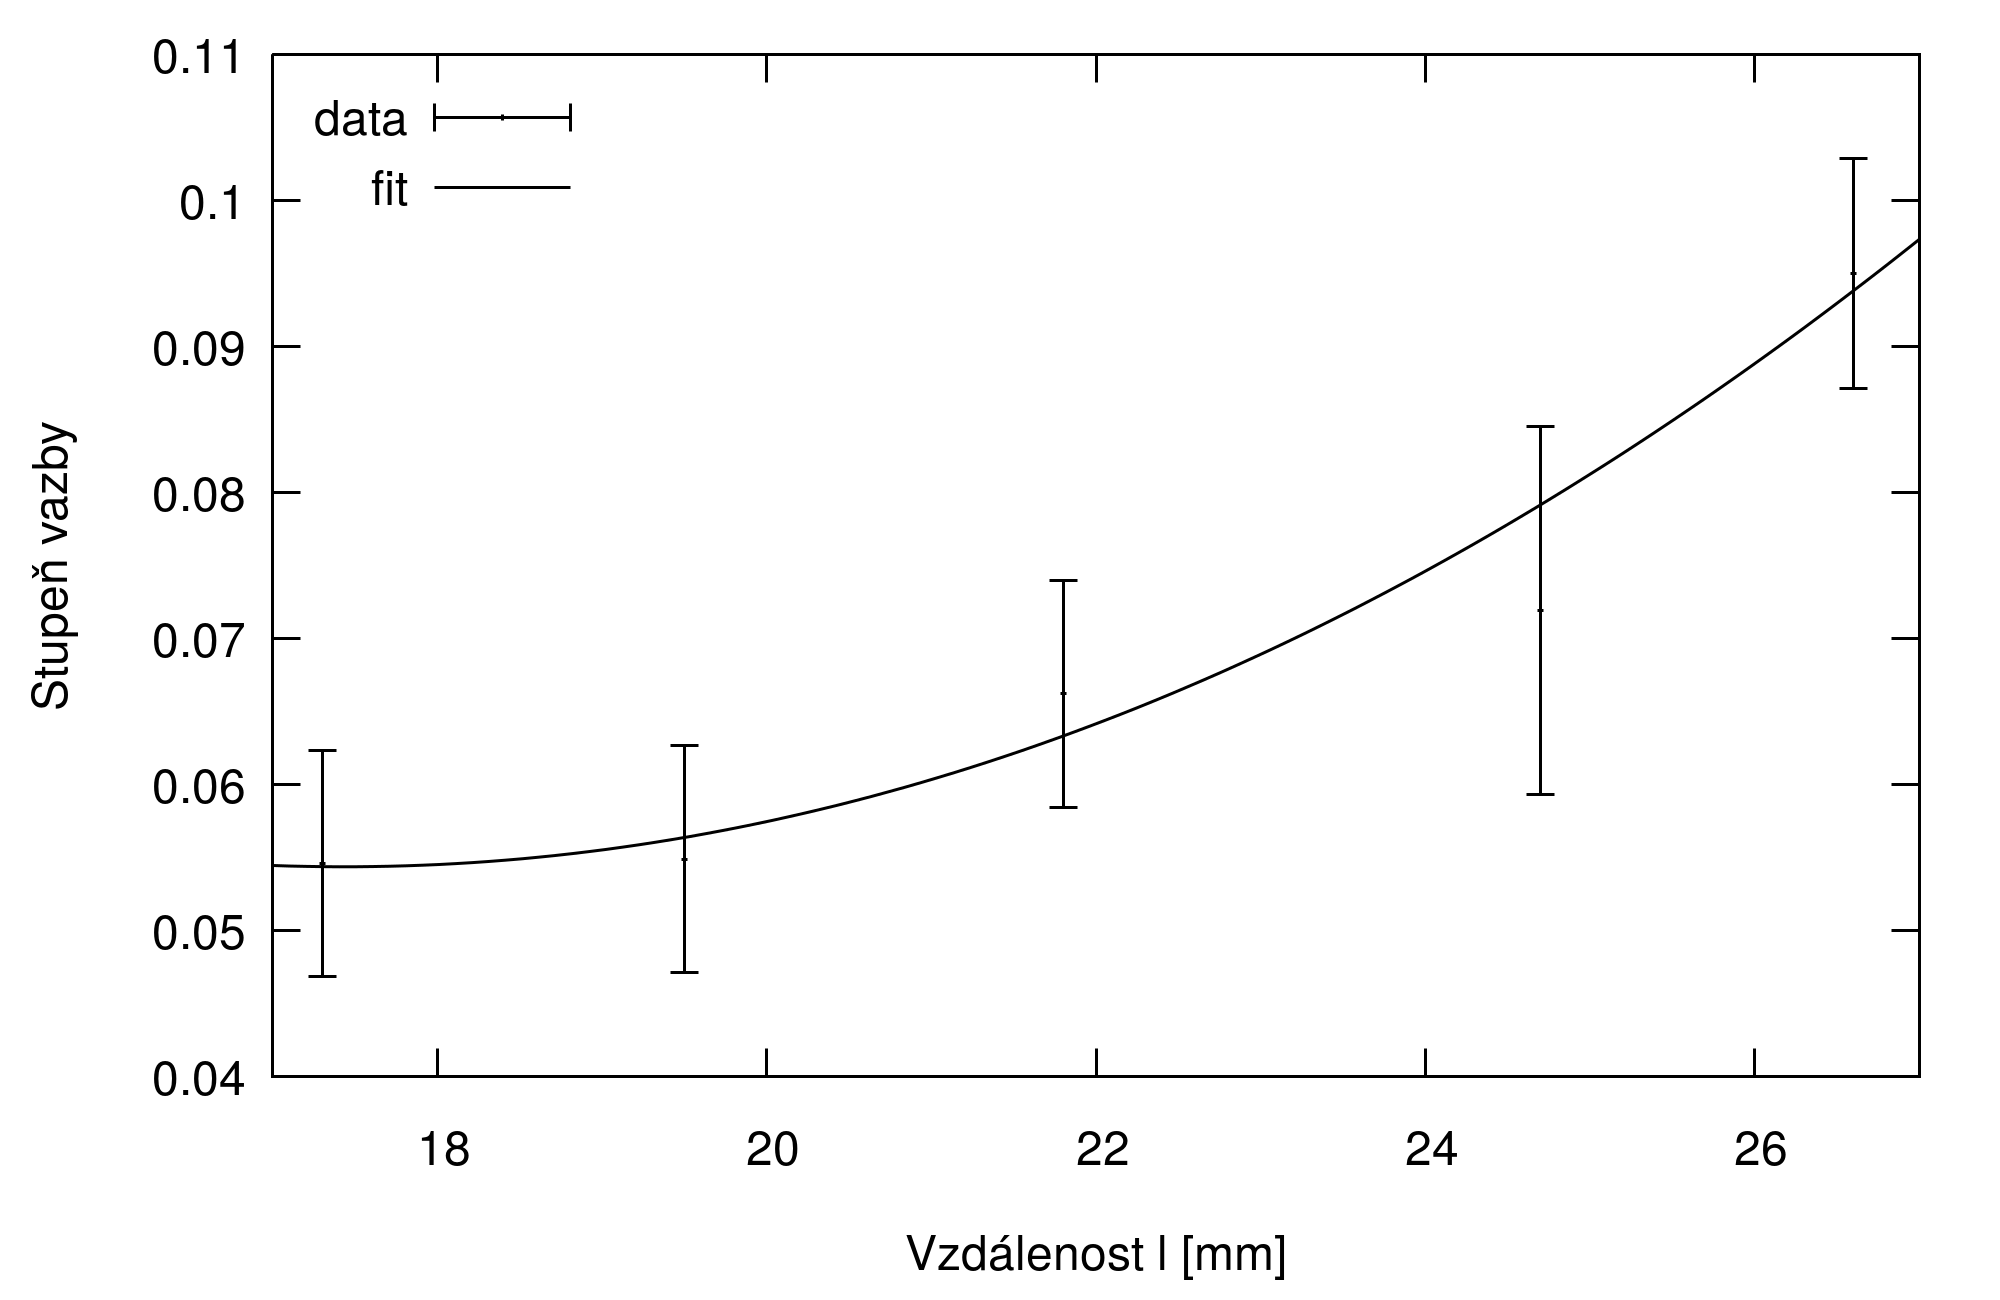
\includegraphics[scale=1.15]{graf}
\caption{Závislost osminásobku periody kmitů reverzního kyvadla na vzdálenosti čočky}
\end{figure}

Směrnice přímky $fit\ dole$ je $k_1 = (0,0062 \pm 0,0002)$, směrnice $fit\ nahore$ $k_2 = (0,0404 \pm 0,0009)$.

\subsection*{Úkol 3}
Dosazením hodnot z tabulky \ref{tab:periody_rev_kyv_2} a hodnoty $l_r$ do \eqref{eq:g_rev_kyv} dostaneme
$$ g = (9,77 \pm 0,02) \ \si{\metre\per\square\second} $$

\subsection*{Úkol 4}
Použitím hodnot z tabulky \ref{tab:delka_provazku}, \ref{tab:rozmer_kulicky} a \eqref{eq:I_fyz_kyv} a hodnot $m_k$ a $m_t$ získáme moment setrvačnosti fyzikálního kyvadla 
$$ I = (0,0632 \pm 0,0003) \ \si{\kilo\gram\metre\squared} $$
Dosazením do \eqref{eq:g_fyz_kyv} dostaneme
$$ g = (9,74 \pm 0,04) \ \si{\metre\per\square\second}.$$
Nepřesnost aproximace fyzikálního kyvadla jako matematického je tedy v rámci chyby měření.

\subsection*{Úkol 5}
Využitím \eqref{eq:teziste_kyv} získáme vzdálenost těžiště fyzického kyvadla od osy otáčení
$$ l_s = 1005,7 \ \si{\milli\metre}$$
Délka matematického kyvadla je 
$$ l_m = L + R = 1010,2 \ \si{\milli\metre} $$
Rozdíl je tedy $4,5 \ \si{\milli\metre}$.

\end{document}
